\documentclass{article}

\usepackage{arxiv}

\usepackage[utf8]{inputenc} % allow utf-8 input
\usepackage[T1]{fontenc}    % use 8-bit T1 fonts
\usepackage{lmodern}        % https://github.com/rstudio/rticles/issues/343
\usepackage{hyperref}       % hyperlinks
\usepackage{url}            % simple URL typesetting
\usepackage{booktabs}       % professional-quality tables
\usepackage{amsfonts}       % blackboard math symbols
\usepackage{nicefrac}       % compact symbols for 1/2, etc.
\usepackage{microtype}      % microtypography
\usepackage{lipsum}
\usepackage{graphicx}

\title{\myTitleMainTitle}

\author{
    Dr Paul J. Palmer
    \thanks{Thanks for everyone who helped.}
   \\
    Author and Determination \\
    Microscope ID Club \\
  Leicestershire VC55 \\
  \texttt{\href{mailto:palmerpjp@gmail.com}{\nolinkurl{palmerpjp@gmail.com}}} \\
   \And
    Pete M. Leonard
   \\
    Author and Determination \\
    Microscope ID Club \\
  Leicestershire VC55 \\
  \texttt{\href{mailto:peteleonard72@gmail.com}{\nolinkurl{peteleonard72@gmail.com}}} \\
  }


% Pandoc citation processing
\newlength{\csllabelwidth}
\setlength{\csllabelwidth}{3em}
\newlength{\cslhangindent}
\setlength{\cslhangindent}{1.5em}
% for Pandoc 2.8 to 2.10.1
\newenvironment{cslreferences}%
  {}%
  {\par}
% For Pandoc 2.11+
\newenvironment{CSLReferences}[2] % #1 hanging-ident, #2 entry spacing
 {% don't indent paragraphs
  \setlength{\parindent}{0pt}
  % turn on hanging indent if param 1 is 1
  \ifodd #1 \everypar{\setlength{\hangindent}{\cslhangindent}}\ignorespaces\fi
  % set entry spacing
  \ifnum #2 > 0
  \setlength{\parskip}{#2\baselineskip}
  \fi
 }%
 {}
\usepackage{calc} % for calculating minipage widths
\newcommand{\CSLBlock}[1]{#1\hfill\break}
\newcommand{\CSLLeftMargin}[1]{\parbox[t]{\csllabelwidth}{#1}}
\newcommand{\CSLRightInline}[1]{\parbox[t]{\linewidth - \csllabelwidth}{#1}\break}
\newcommand{\CSLIndent}[1]{\hspace{\cslhangindent}#1}

%\usepackage{booktabs}
%\usepackage{longtable}
%\usepackage{morefloats}
%\extrafloats{100}
%\date{August 25, 2021}
%\renewcommand{\today}{September 5, 2021}

% Set the copyright footer
%\lfoot{\copyright 2021 P.J. Palmer  P.M. Leonard}

% Some figure placement options.
%\usepackage[figuresonly,nomarkers,fighead, figlist]{endfloat}
%\usepackage[figuresonly,nomarkers,nolists]{endfloat}
% Put multiple figures per page
%\renewcommand{\efloatseparator}{\mbox{}}
\usepackage{flafter}
\usepackage{booktabs}
\usepackage{longtable}
\usepackage{array}
\usepackage{multirow}
\usepackage{wrapfig}
\usepackage{float}
\usepackage{colortbl}
\usepackage{pdflscape}
\usepackage{tabu}
\usepackage{threeparttable}
\usepackage{threeparttablex}
\usepackage[normalem]{ulem}
\usepackage{makecell}
\usepackage{xcolor}


\begin{document}
\maketitle

\def\tightlist{}


\begin{abstract}
\myAbstract
\end{abstract}


\hypertarget{introduction}{%
\section{Introduction}\label{introduction}}

\myTitleMainTitle

This report records the determinations made by microscopic examination of Lepidoptera specimens made by VC55 recorders. Specimens were not retained, as each determination is illustrated by micro-photographs of specimens and temporary slides. The high quality micro-photographs were produced by stacked focus photography and are much easier to work with than traditional permanent slides. In most cases, the artificial depth of field provides a better view of dissected parts than can be seen through a microscope. Using micro-photographs has also allowed on-line collaboration using the version management tool GitHub (\url{https://github.com}) to manage this and other reports.

The primary sources for identifying Lepidoptera by dissection used in this work are Hall et al. (2021) and Schön (2021). The determination was also checked against the appearance of the imago using Kimber (2021) amongst other sources.

\hypertarget{species-summary}{%
\section{Species Summary}\label{species-summary}}

The species recorded are presented in Table \ref{tab:TableSpeciesList} which has been directly generated from the records.

\begin{longtable}[t]{lllr}
\caption{\label{tab:TableSpeciesList}Species recorded by family and gender.}\\
\toprule
family & taxon & gender & Count\\
\midrule
\endfirsthead
\caption[]{\label{tab:TableSpeciesList}Species recorded by family and gender. \textit{(continued)}}\\
\toprule
family & taxon & gender & Count\\
\midrule
\endhead

\endfoot
\bottomrule
\endlastfoot
\cellcolor{gray!6}{Shrekidae} & \cellcolor{gray!6}{Shrekus greenus} & \cellcolor{gray!6}{Male} & \cellcolor{gray!6}{1}\\*
\end{longtable}

A total of 1 specimens were examined of which 1 were identified.

\begin{figure}[p]

{\centering \includegraphics{dissection-report_files/figure-latex/unnamed-chunk-8-1} 

}

\caption{Map of all records by tetrad.}\label{fig:unnamed-chunk-8}
\end{figure}

\begin{figure}[p]

{\centering \includegraphics{dissection-report_files/figure-latex/unnamed-chunk-9-1} 

}

\caption{Phenology of all records.}\label{fig:unnamed-chunk-9}
\end{figure}

\newpage

\hypertarget{dummyidea-records}{%
\section{Dummyidea Records}\label{dummyidea-records}}

\hypertarget{specimen-dummy-ogre}{%
\subsection*{\texorpdfstring{Specimen dummy \emph{ Shrekus greenus } Ogre}{Specimen dummy  Ogre}}\label{specimen-dummy-ogre}}
\addcontentsline{toc}{subsection}{Specimen dummy \emph{ Shrekus greenus } Ogre}

\textbf{Label details:}
record.date: 2022-01-01, site: Far far away, VC: 1024, grid.ref: SK75651803, recorder.name: Shrek, comments: Very swampy, determiner: Prince Charming, method: Mace, stage: Ogre, quantity: 1, order: Dummyidea, family: Shrekidae, sub.family: None, genus: shrekus, taxon: Shrekus greenus, log.number: 1000032, Code: 000000, vernacular: Ogre, and gender: Male.

\begin{figure}[p]

{\centering 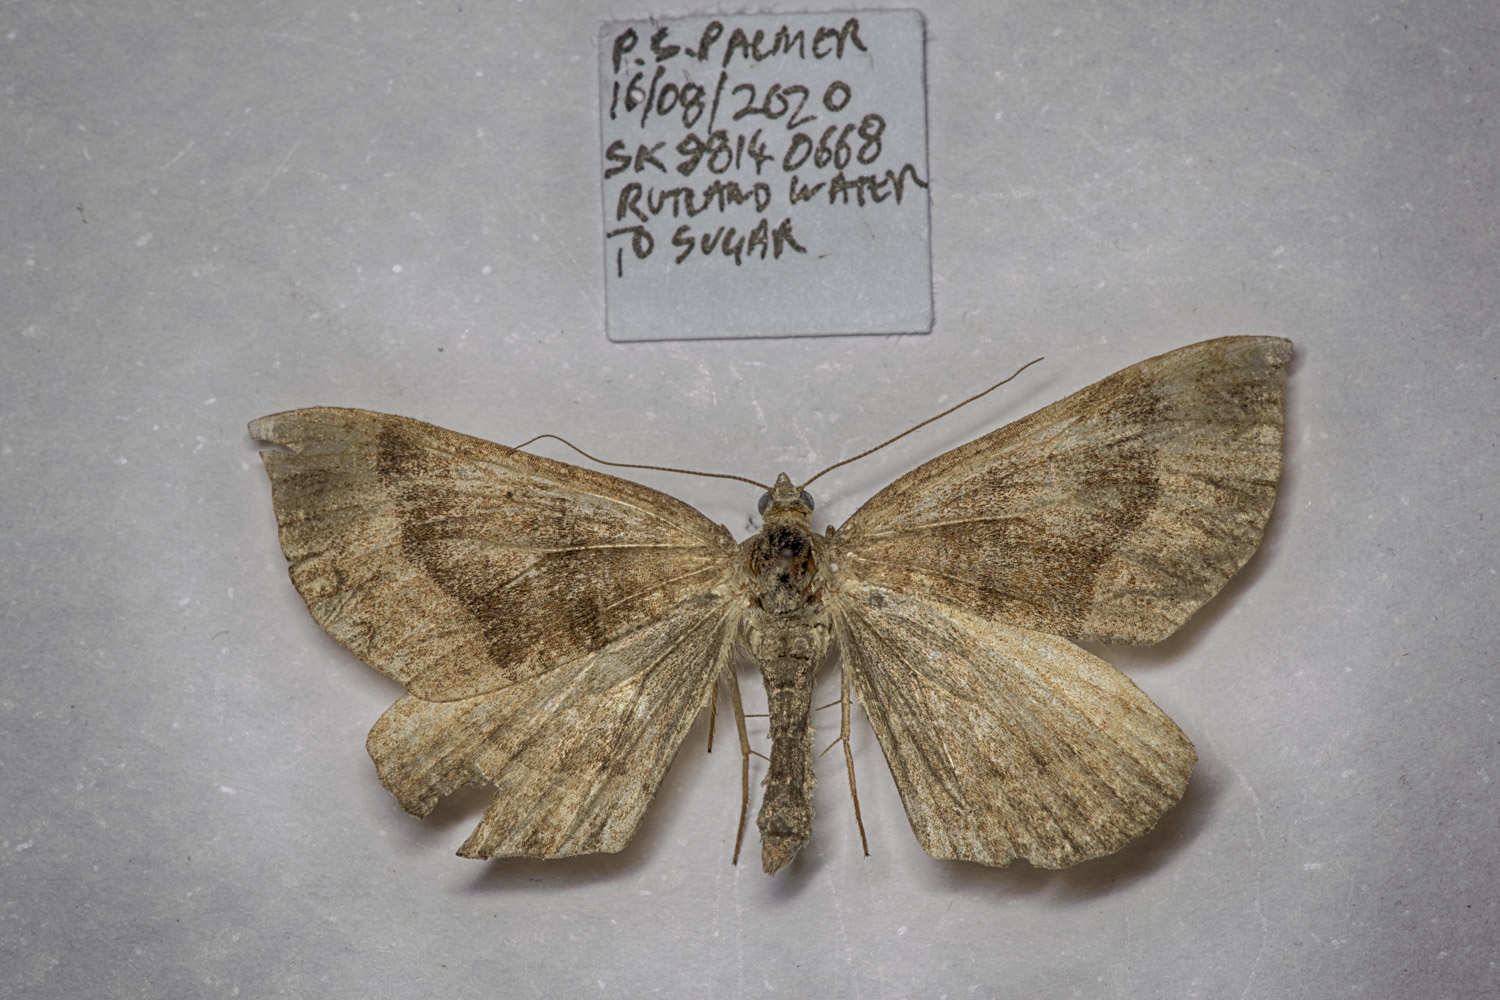
\includegraphics[width=2.14in]{/Users/TechTrends/Documents/my_github/Packages/bookdown-report/_records/dummy-records-delete/dummy/images/202009131026PJP-1} 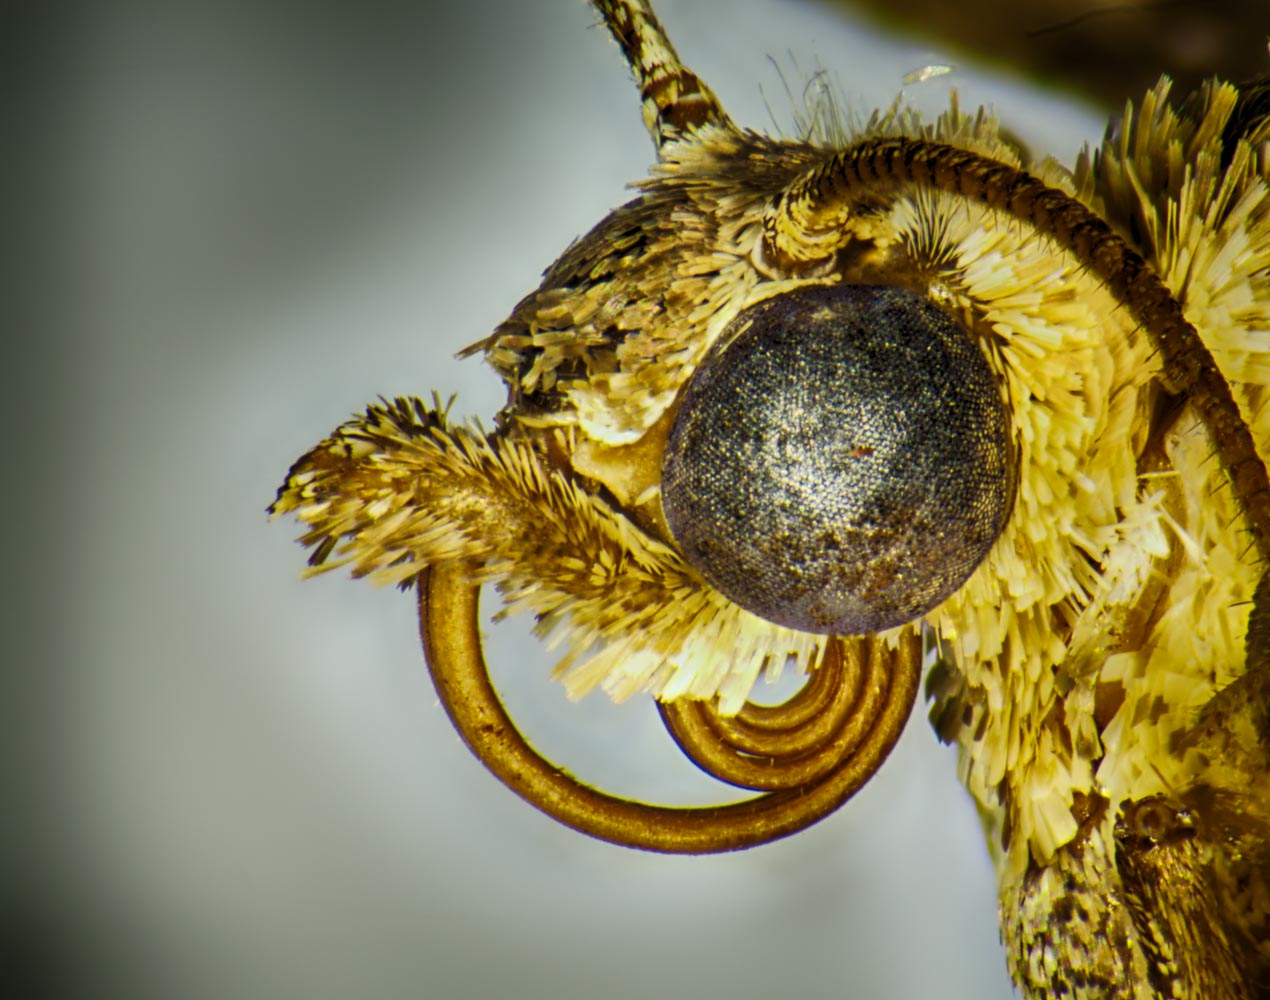
\includegraphics[width=1.81in]{/Users/TechTrends/Documents/my_github/Packages/bookdown-report/_records/dummy-records-delete/dummy/images/20201112-1} 

}

\caption{dummy  \emph{ Shrekus greenus } Ogre dummy  \emph{ Shrekus greenus } Ogre Specimen images}\label{fig:unnamed-chunk-16}
\end{figure}

\hypertarget{dissection}{%
\subsection{Dissection}\label{dissection}}

\begin{figure}[p]

{\centering 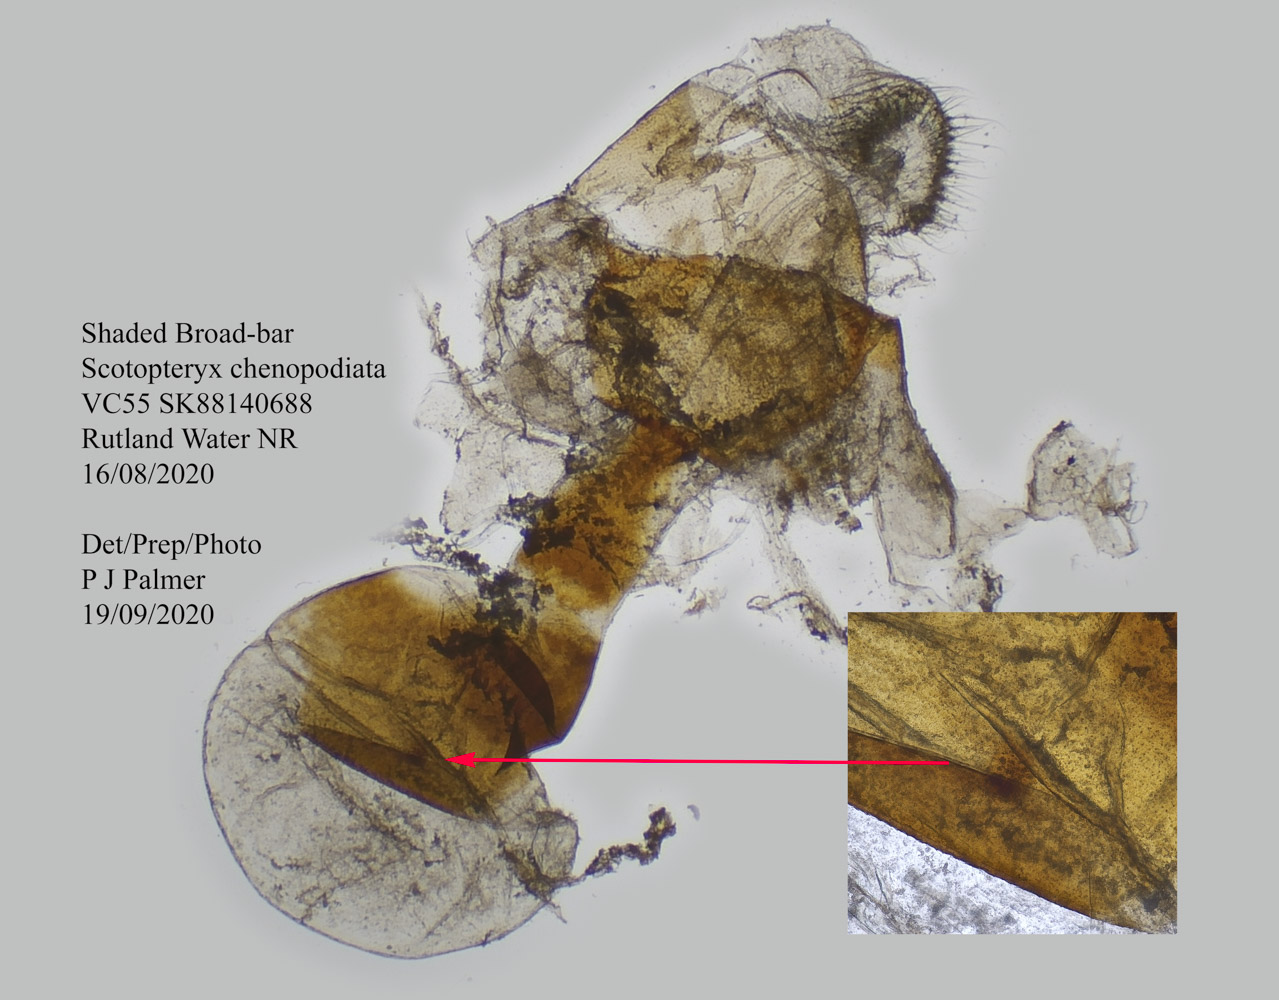
\includegraphics[width=1.83in]{/Users/TechTrends/Documents/my_github/Packages/bookdown-report/_records/dummy-records-delete/dummy/images/dissection/202009131026PJP-3} 

}

\caption{dummy  \emph{ Shrekus greenus } Ogre temporary slide in Hoyers}\label{fig:unnamed-chunk-17}
\end{figure}

\hypertarget{references}{%
\section*{References}\label{references}}
\addcontentsline{toc}{section}{References}

\hypertarget{refs}{}
\begin{CSLReferences}{1}{0}
\leavevmode\hypertarget{ref-Hall2021}{}%
Hall, Peter, Patrick Clement, Jon Clifton, Mike Dale, and Rachel Terry. 2021. {``{Moth Dissection UK}.''} \url{https://mothdissection.co.uk}.

\leavevmode\hypertarget{ref-Kimber2021}{}%
Kimber, Ian. 2021. {``{UK Moths}.''} \url{https://ukmoths.org.uk}.

\leavevmode\hypertarget{ref-Schon2021}{}%
Schön, Walter. 2021. {``{Lepiforum}.''} \url{http://lepiforum.org/}.

\end{CSLReferences}

\let\cleardoublepage\clearpage

\bibliographystyle{unsrt}
\bibliography{references.bib}


\end{document}
